
% Our architecture for implementing security metrics is straight forward. We declare a \textit{base security metric} type from which all metrics inherit three methods: 
% \begin{itemize}
% \item CheckPreReqs: is invoked either directly by the caller or in the calculate method to ensure all items necessary for the calculation are present.
% \item Calculate: returns the resulting measurement
% \item GetMetadata: returns the environment and ancillary data used during the calculation 
% \end{itemize}
 
\begin{figure}[H]
\centering
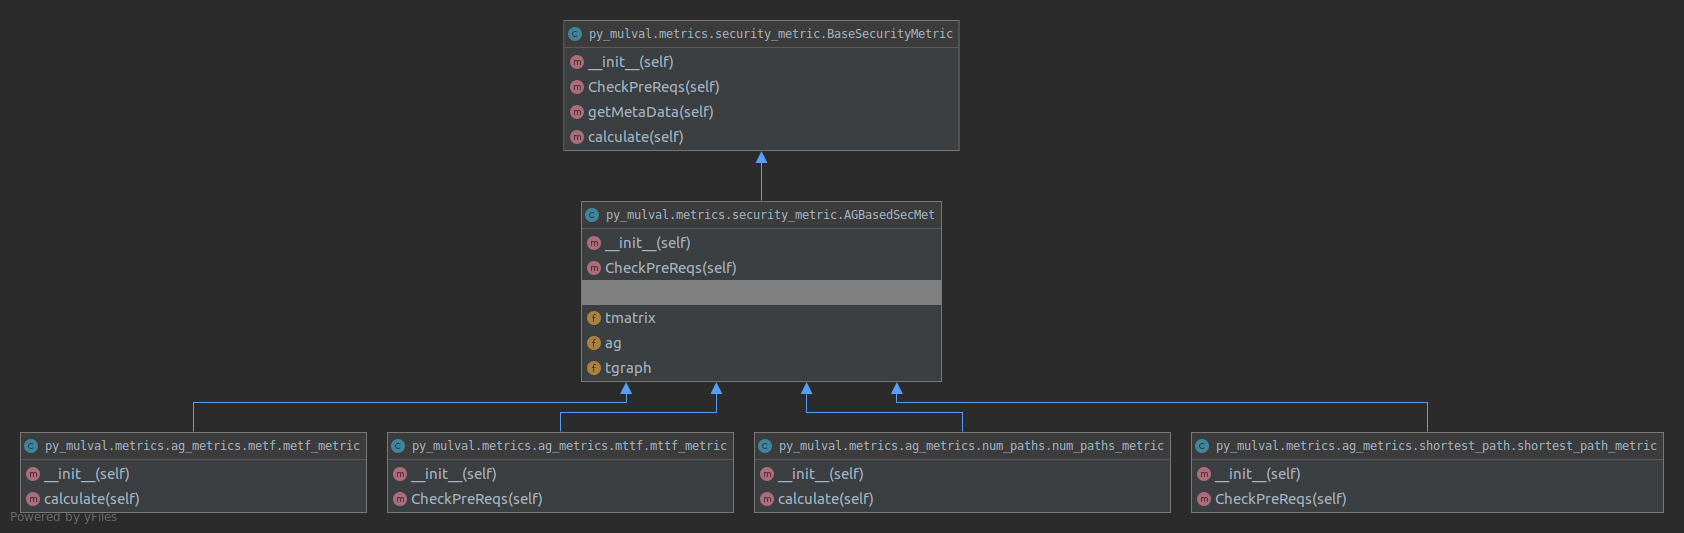
\includegraphics[width=.95\linewidth]{resource/img/ch_automation/metrics_class_uml.png}
\caption{Metric Class Diagram}
\label{fig:automation:metric_uml}
\end{figure} 

Figure \ref{fig:automation:metric_uml} shows the inheritance hierarchy for attack graph based security metrics. Each AG metric implementation inherits from AGBasedSecMetric which in turn inherits from BaseSecurityMetric. AGBasedSecMetric includes a property for attack graph which is a requirement to perform the metric calculation. Each BaseSecurityMetric also contains immutable properties for the name of the metric, the expected measurement unit for results, a citation field linking to the source paper where we found the metric, and a short summary of what the metric does. All these properties plus any additional information derived during calculation are added to the metadata dictionary of the metric and returned when the calculate method is called. 


\begin{figure}[H]
\centering
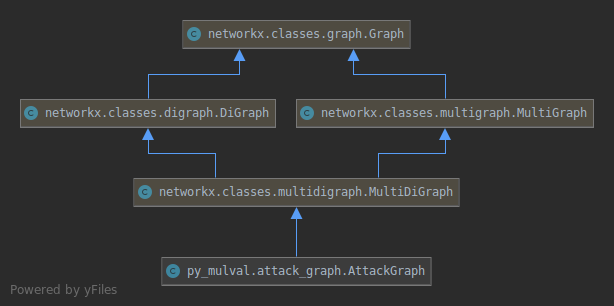
\includegraphics[width=.95\linewidth]{resource/img/ch_automation/attack_graph_simple_uml.png}
\caption{Attack Graph Class Diagram}
\label{fig:automation:ag_uml}
\end{figure} 

% The attack graphs described in the literature vary somewhat in structure among implementations. For example, the AGs presented in \cite{Ou_Appel_2005} include non-exploits along with exploits as nodes with edges representing lateral movements. In \cite{Noel_Jajodia_2014} the non-exploit nodes don't appear to be present in the publication, although the TVA tool isn't publicly available to test this. In \cite{Dacier_1994} and \cite{Ortalo_1999} nodes represent system privileges and edges contain exploits that grant an attacker additional privileges on a set of systems, while in \cite{Phillips_Swiler_1998} edges carry probabilities of exploitation and the nodes represent actual hosts. While the differences are subtle, they are enough to necessitate a general form of attack graph which we present in Figure \ref{fig:automation:ag_uml}. Our representation of an attack graph is a multi-edged directed acyclic graph.     

% \begin{wrapfigure}[10]{I}{.25\textwidth}
\begin{figure}[H]
\centering
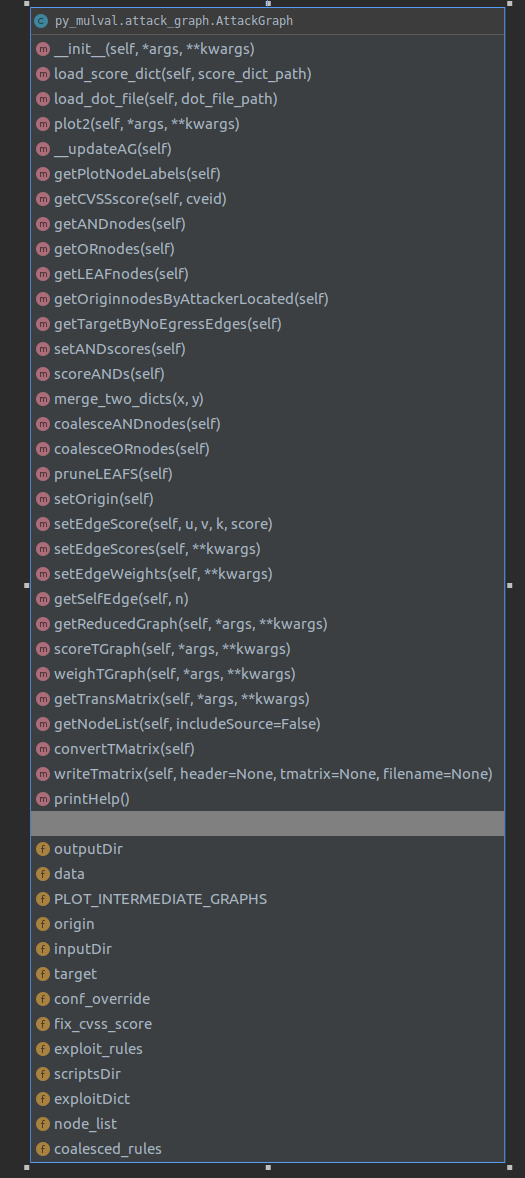
\includegraphics[scale=.45]{resource/img/ch_automation/attack_graph_class_diag.png}
% \end{wrapfigure}
\caption{Attack Graph Methods and Properties}
\label{fig:automation:ag_details_uml}
\end{figure}

As shown in Figure \ref{fig:automation:ag_details_uml}, our implementation allows us to load various AG formats from graph description language (.dot) files, from adjacency lists as shown in Tables \ref{tab:eg_verts} and \ref{tab:eg_arcs}, or other formats as specified. Once loaded, we provide programmatic access to manipulate scoring and weighting functions, exploits definitions, and vulnerability scores. 
% This allows for a simple means to test the range of values a metric will generate, the sensitivity of a metric to fluctuations in parameters, and how well a metric performs on different models. It also gives us some insights into how well each AG type actually models threat and defense attributes.


% In the \textit{Input} stage of Figure \ref{fig:automation:metric_pipeline}, system details depicted above the inbound arrows on the left are parsed into a model which describes the current environment or environment under test. Model parameters can be populated synthetically or from a live system. Rules comprising the threat model which describes how these components are allowed to interact with each other and with external stimulus can be added here for metrics that require it. The raw inputs to the processing pipeline can vary widely depending on which security metrics are being considered. At a high level, we treat the input stage as a black box for handling information requests from subsequent stages. This affords us the freedom to connect static data for testing and experimentation, and live data for production deployments without altering the contract or interface. In practice input targets can be existing APIs provided by SIEMs, query interfaces to a configuration database, source code repositories, vulnerability information feeds, generated network topologies, etc. At this stage we only assume appropriate adapters exist to make this data available for the subsequent stages.

% The \textit{Pre Process} stage transforms the current knowledge base into a format suitable for the desired metric calculation. 

% \begin{figure}[ht]
% \centering
% \includegraphics[width=.5\linewidth]{resource/img/ch_benchmarking/secmet_ptah/Ptah_archs.png}
% \caption{Preprocessing and Transformation Handlers (\textbf{PTaH})}
% \label{fig:automation:ptah_arch}
% \end{figure} 

In order to experiment with different network architectures and exploit effects, it was necessary to reproduce each step in the process: 
Install AG suite (MulVal, XSB) $\rightarrow$ Define AG input model (Datalog/Prolog) $\rightarrow$ Generate AG (Java, C++, ANTLR4, sed) $\rightarrow$ Import NVD (JSON, XML $\rightarrow$ SQL) $\rightarrow$ Implement custom adaptor for Stochastic Model expected input (Python, inference) $\rightarrow$ Insert transition matrix into provided R script (ctrl+c, ctrl+v) 
After following this process precisely 2 times we understood why the AG based analytics community isn’t larger. Our immediate solution was to create a set of ansible roles and plays to automate the environment setup, test execution, and results collection entirely with a single command. This in itself lowers the barrier to entry for anyone interested in experimenting with attack graphs or looking to (quickly) reproduce our results.

% \begin{figure}[ht]
% \includegraphics[width=.48\textwidth]{img/Ptah_archs.png}
% \caption{Preprocessing and Transformation Handlers (\textbf{PTaH})}
% \label{fig:automation:ptah_arch}
% \end{figure} 


To handle the scale and volume of requests needed to support the advanced use-cases listed below, we are currently implementing and evaluating the following features in the SMaaS architecture:
Metric Isolation: Each metric should be independently deployable to allow scaling up and down as request volume dictates. Currently metrics are bundled in Python and R modules with logical separation at the function level.


The \textit{Compute} stage implements the calculation of the security metric and takes the measurement of the current state. 

The surveys covered in Section \ref{sec:background:metrics} describe properties common to all the security metrics they consider, which become evaluation criteria for their review. All security metrics inherit from a parent metric class that defines these common properties and the current system model, along with housekeeping functions and metadata like citations and usage.The security metric does not contain logic to create the inputs it operates on, so we can stack metrics to run in parallel against a single source of facts, or chain them in a processing pipeline to compose more complex analytics. 



% Finally, the \textit{Reporting} stage handles the response logic needed to return the measured value and associated metadata appropriately. In our experience, most security metrics return a single value, although heuristics are also supported as bucket sizes and value count arrays returned within the accompanying metadata. 

% In order to experiment with different network architectures and exploit effects, it was necessary to reproduce each step in the process: 
% Install AG suite (MulVal, XSB) $\rightarrow$ Define AG input model (Datalog/Prolog) $\rightarrow$ Generate AG (Java, C++, ANTLR4, sed) $\rightarrow$ Import NVD (JSON, XML $\rightarrow$ SQL) $\rightarrow$ Implement custom adaptor for Stochastic Model expected input (Python, inference) $\rightarrow$ Insert transition matrix into provided R script (ctrl+c, ctrl+v) 
% After following this process precisely 2 times we understood why the AG based analytics community isn’t larger. Our immediate solution was to create a set of ansible roles and plays to automate the environment setup, test execution, and results collection entirely with a single command. This in itself lowers the barrier to entry for anyone interested in experimenting with attack graphs or looking to (quickly) reproduce our results.

% \begin{figure}[ht]
% \includegraphics[width=.48\textwidth]{img/Ptah_archs.png}
% \caption{Preprocessing and Transformation Handlers (\textbf{PTaH})}
% \label{fig:automation:ptah_arch}
% \end{figure} 


% To handle the scale and volume of requests needed to support the advanced use-cases listed below, we are currently implementing and evaluating the following features in the SMaaS architecture:
% Metric Isolation: Each metric should be independently deployable to allow scaling up and down as request volume dictates. Currently metrics are bundled in Python and R modules with logical separation at the function level.




